La sfida a cui ho accettato di sottopormi, consiste in un importante problema di pangenomica computazionale, ovvero quello di costruire, in linguaggio Rust, uno splicing graph  a partire da un allineameto multiplo di trascritti di un gene fornito in input. 

Prima di esporre la soluzione al problema, saranno necessari alcuni concetti preliminari, quali quelli di \textit{Allineamento Multiplo} e \textit{Splicing Graph}. Nozioni come \textit{Hugo Name} o \textit{Trascritto} sono già stati forniti nel capitolo \ref{chap:comp_bio}.

\section{Allineamento di Sequenze}
In generale, un allineamento di sequenze è una procedura bioinformatica con cui vengono messe a confronto ed allineate due o più sequenze primarie di aminoacidi, DNA o RNA. L'allineamento permette di individuare regioni identiche o simili che possono avere relazioni funzionali, strutturali o filogenetiche (evolutive). Spesso l'allineamento viene utilizzato per verificare se una sequenza di interesse sia presente all'interno di un database di sequenze conosciute oppure se ne esista una simile. 

Nel caso ristretto dell'allineamento tra due sequenze, quest'ultimo estende il concetto di \textit{Distanza di Hamming} a strighe di lunghezza diversa.

La Distanza di Hamming è definita, solo su strighe di uguale lunghezza, come il numero di posizioni nelle quali i simboli corrispondenti in due stringhe $s_1$ ed $s_2$ divergono. 

In simboli, per distanza, si intende una funzione $d: \mathbb{S}\times \mathbb{S} \to \mathbb{R_+}$, dove $\mathbb{S}$ è l'insieme delle stringhe, che abbia tre proprietà : 

\begin{itemize}
    \item \textsc{Riflessività:} $d(x,y)=0 \iff x=y \textrm{ } \forall \textrm{ } x,y \in \mathbb{S}$
    \item \textsc{Simmetria:} $d(x,y)=d(y,x) \textrm{ } \forall \textrm{ } x,y \in \mathbb{S}$
    \item \textsc{Disuguaglianza Triangolare:} $d(x,y) +d(y,z)\geq d(x,z), \textrm{ } \forall \textrm{ } x,y,z \in \mathbb{S}$
\end{itemize}

Per fare in modo di poter allineare due stringhe con lunghezze diverse, vengono introdotti gli \textit{Indel} (-), che hanno la funzione di "Riempire i buchi". Ci sono due restrizioni nell'iserimento degli indel:

\begin{itemize}
    \item Non possono esistere colonne di soli indel
    \item Le strinche estese di Indel devono avere la stessa lunghezza
    \label{itemize:indel_cond}
\end{itemize}

\begin{example}
$s_1=ABRACADABRA,s_2=BANANA$ \\
Alcuni possibili allineamenti sono:
    \begin{center}
      \begin{tabular}{ c c c c c c c c c c c}
        A & B & R & A & C & A & D & A & B & R & A \\ 
        - & B & - & A & N & A & - & - & - & N & A \\ \hline
        A & B & R & A & C & A & D & A & B & R & A \\ 
        - & - & - & B & - & A & N & A & - & N & A \\ \hline
        A & B & R & A & C & A & D & A & B & R & A \\ 
        - & B & A & N & A & - & - & - & - & N & A \\
      \end{tabular}
    \end{center}
Ciò non significa che siano tutti ugualmente \textit{buoni}
\end{example}

Per saggiare la bontà di un allineamento, è necessario formalizzarlo come un problema di ottimizzazione, quindi definendo:

\begin{itemize}
    \item \textsc{Insieme delle stanze:} Un elemento di $\mathbb{S}\times \mathbb{S}$
    \item \textsc{Insieme delle Soluzioni ammissibili:} gli allineamenti che rispettano le condizioni elencate precedentemente 
    \item \textsc{Funzione Obiettivo:} $\sum_{i=1}^{l} score(s_1[i],s_2[i])$
    \item \textsc{Soluzione:} Allineamento che massimizza l'omologia, quindi la funzione obiettivo
\end{itemize}

Dove $score(s_1[i], s_2[j])$ è il valore del'incolonnamento della colonna presa in esame. Questo valore può essere prelevato da opportune \textit{Matrici di Score} che contengono una funzione $score(c_1, c_2)$ per ogni carattere dell'alfabeto in questione. Ad esempio una matrice di score potrebbe essere \textsc{BLOSUM62} e l'alfabeto $\Sigma=\{A, C, G, T\}$.

\begin{figure}
    \centering
    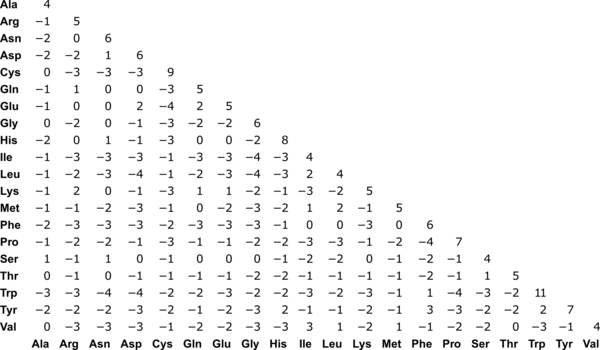
\includegraphics[scale= 0.5]{images/BLOSUM62.png}
    \caption{La matrice di score \textsc{BLOSUM62}}
    \label{fig:blosum32}
\end{figure}

In breve un allineamento può essere interpretato come una misura di omologia tra due o più sequenze. I mismatches possono essere interpretati come punti di mutazione tra le sequenze, invece gli indel o le sequenze di indel (GAP) possono essere interpretate come punti di divergenza nelle sequenze genomiche 

\section{Algoritmi di Allineamento}
Esistono due principali algoritmi che performano allineamenti:  l'algoritmo di Needleman-Wunsch che performa un allineamento globale, cioè allinea le sequenze nella loro interezza e l'algoritmo di Smith-Waterman, che invece performa un allineamento locale, cioè evidenzia regioni simili nelle sequenze genomiche.

\subsection{Algoritmo di Needleman-Wunsch}
L'algoritmo di Needleman-Wunsch utilizza un approccio di programmazione dinamica per risolvere il problema e definisce una equazione di ricorrenza struttutata nel seguente modo : 

\begin{equation*}
    M[i, j] = \textrm{allineamento  ottimo  su }  s1[:i],  s2[:j]
\end{equation*}

\begin{equation}
    M[i, j] = \max  {
                    \begin{cases} 
                        M[i \textrm{-} 1,j \textrm{-} 1] +d(s1[i],s2[j]) & \textrm{nessun indel}\\
                        M[i,j \textrm{-} 1] +d(\textrm{-},s2[j]) & \textrm{indel solo in } s_1\\
                        M[i \textrm{-} 1,j] +d(s1[i],\textrm{-}) & \textrm{indel solo in } s_2\\
                    \end{cases}
                    }
\end{equation}

dove $d(s1[i],s2[j])$ è il punteggio ottenuto dalla matrice di score. Si ricoda che non è contemplato il caso di soli indel in colonna.

Le condizioni al contorno sono:

\begin{itemize}
    \item $M[0,0]=0$
    \item $M[i,0]=M[i \textrm{ - } 1,0] + d(s_1[i],-)$
    \item $M[0,j]=M[0,j \textrm{ - } 1] + d(-,s_2[j])$
\end{itemize}

Il tempo di esecuzione è $\mathcal{O}(nm)$ dove $|s_1|=n$ e $|s_2|=m$.

L'allineamento può essere ottenuto tramite l'usuale \textit{TraceBack} della matrice di programmazione dinamica, partendo da $M[n,m]$ retrocedendo fino a $M[0,0]$.

\begin{figure}[ht]
    \centering
    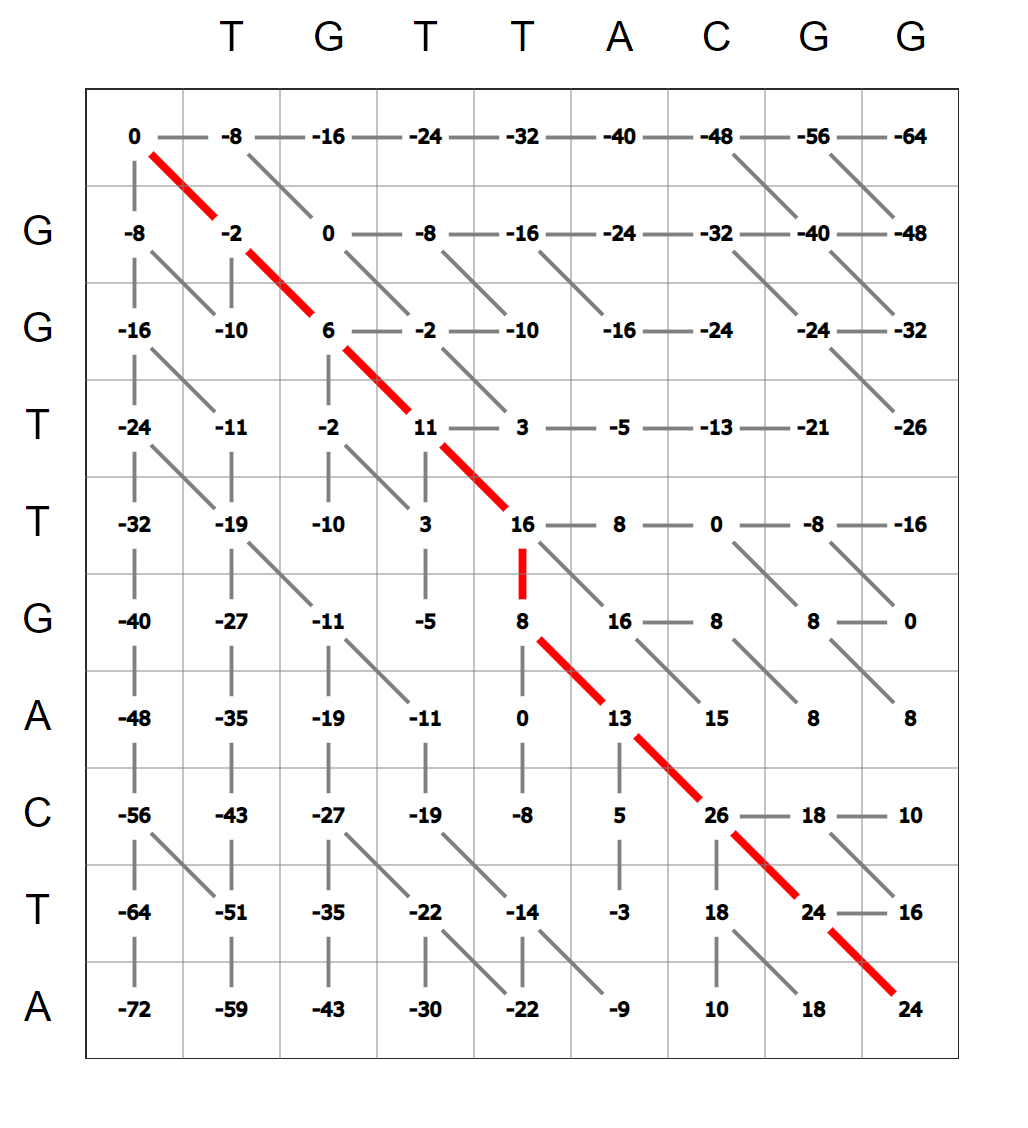
\includegraphics[scale=0.45]{images/esempio nw.PNG}
    \caption{Esempio di esecuzione dell'algoritmo di Needleman-Wunsch su istanza : $s_1=TGTTACGG$ e $s_2=GGTTGACTA$}
    \label{fig:nw}
\end{figure}

\subsection{Algoritmo di Smith-Waterman}
L'algoritmo di Smith-Waterman, come quello di Needleman-Wunsch, utilizza un approccio di programmazione dinamica, ma a differenza di quest'ultimo, evidenzia le sottostringhe di $s_1$ ed $s_2$ che massimizzano il punteggio di allineamento. In altre parole cerca di trovare $t_1=s_1[h:i]$ e $t_2=s_2[k:j]$ tale che il punteggio di allineamento di $t_1$ e $t_2$ sia massimo.

Per raggiungere questo obiettivo pone un limite inferiore al punteggio di allineamento, che non può essere negativo, aggiungendo un nuovo caso all'equazione di ricorrenza dell'algoritmo di Needleman-Wunsch, che si modifica nel seguente modo:

\begin{equation*}
    M[i, j] = \textrm{allineamento  ottimo  su }  s1[:i],  s2[:j]
\end{equation*}

\begin{equation}
    M[i, j] = \max  {
                    \begin{cases} 
                        0\\
                        M[i \textrm{-} 1,j \textrm{-} 1] +d(s1[i],s2[j]) & \textrm{nessun indel}\\
                        M[i,j \textrm{-} 1] +d(\textrm{-},s2[j]) & \textrm{indel solo in } s_1\\
                        M[i \textrm{-} 1,j] +d(s1[i],\textrm{-}) & \textrm{indel solo in } s_2\\
                    \end{cases}
                    }
\end{equation}

dove $d(s1[i],s2[j])$, come in Needleman-Wunsch, è il punteggio ottenuto dalla matrice di score.

Le condizioni al contorno sono differenti da quelle dell'algoritmo di Needleman-Wunsch, in quanto un allineamento non può avere punteggio negativo, e si modificano come segue:

\begin{itemize}
    \item $M[0,0]=0$
    \item $M[i,0]=0 \textrm{ } \forall i \textrm{ } | \textrm{ } 1\leqslant i \leqslant n$
    \item $M[0,j]=0 \textrm{ } \forall j \textrm{ }| \textrm{ } 1\leqslant j \leqslant m$
\end{itemize}

Il tempo di calcolo, come in Needleman-Wunsch, è $\mathcal{O}(nm)$ dove $|s_1|=n$ e $|s_2|=m$.

Il Traceback diventa però più complicato, in quanto deve essere effettuato dal valore massimo della matrice di programmazione dinamica, retrocedendo fino al primo 0.

\begin{figure}[ht]
    \centering
    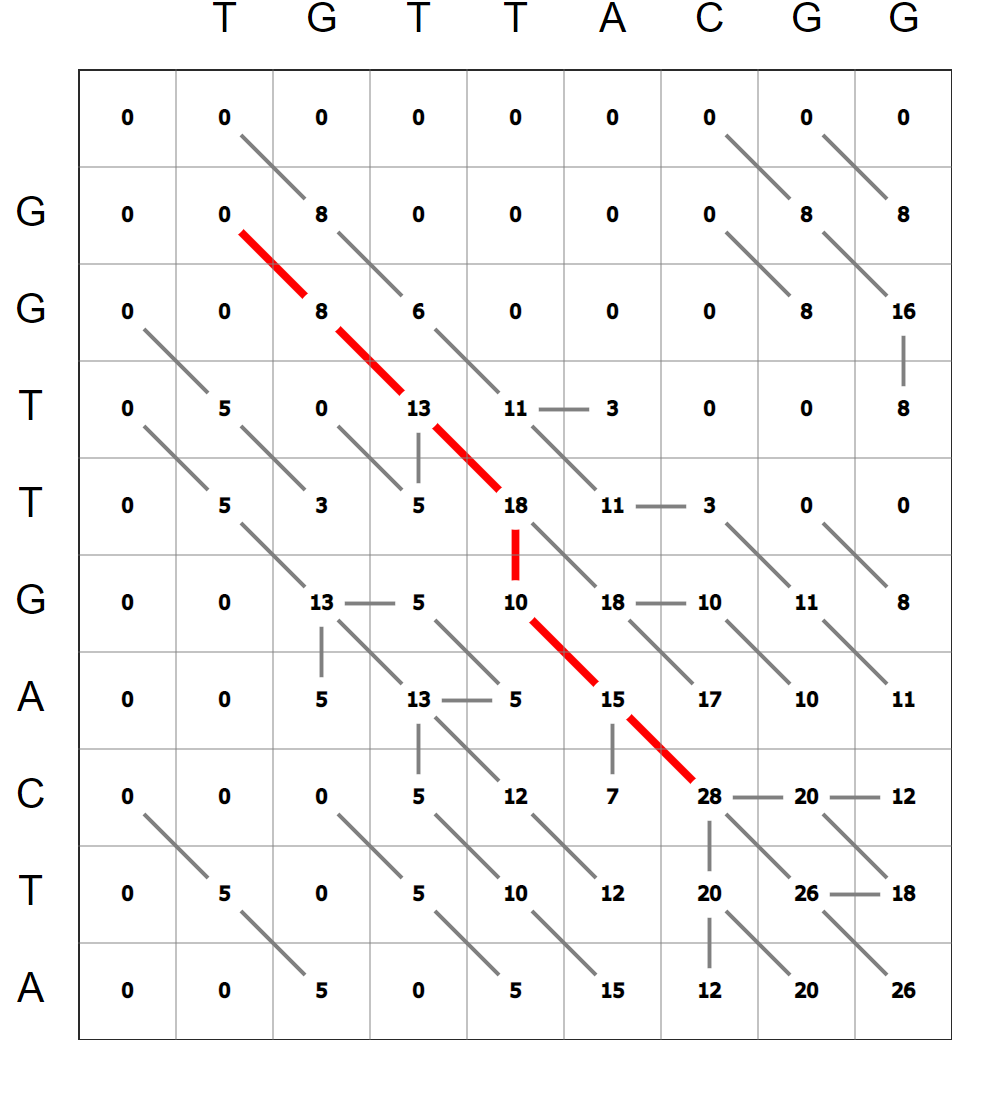
\includegraphics[scale=0.45]{images/esempio sw.PNG}
    \caption{Esempio di esecuzione dell'algoritmo di Smith-Waterman sulla stessa istanza della figura \ref{fig:nw}}
    \label{fig:sw}
\end{figure}

\clearpage
\section{Allineamento multiplo di sequenze}

L'allineamento multiplo è un'esensione del problema dell'allineamento di due sequenze, infatti, l'istanza del problema non sono più due sole strighe, ma un insieme di $k$ stringhe $\mathbb{S}=\{s_1,s_2,s_3,..,s_k\}$.

\begin{figure}[ht]
    \centering
    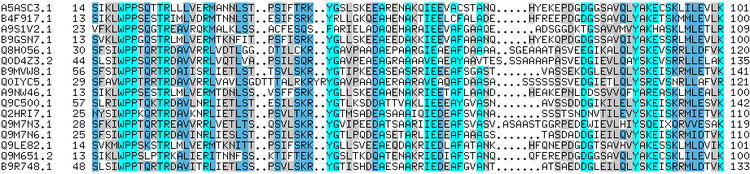
\includegraphics[scale=0.5]{images/multiple sequence alignment.png}
    \caption{Esempio di allineamento multiplo tra sequenze}
    \label{fig:mul_al}
\end{figure}

Ciò però introduce alcuni problemi, ad esempio come posizionare gli indel nelle colonne dell'allineamento. Sicuramente ci potranno essere più indel in una singola colonna, ma non solamente indel, infatti è possibile accettarne fino a $k-1$.

Un altro problema è la funzione codificata nella matrice di score. Infatti essa è una funzione definita $score: \Sigma \times \Sigma \to \mathbb{R_+}$, dove $\Sigma$ è l'alfabeto dei simboli delle stringhe, perciò non può restituire un valore per un numero arbitrario di strighe.

Questo problema è risolto utilizzando la funzione \textit{Sum of Pairs} che somma il punteggio di tutte le righe, prese a coppie, in una colonna di allineamento e ne fa la somma.

Una possibile soluzione al problema dell'allineamento multiplo, è un algoritmo di programmazione dinamica. Questa volta però, a differenza dei due precedenti, l'ultima componente dell'allineamento può trovarsi in $2^k-1$ casi (non è possibile il caso di soli indel).

Il tempo di calcolo è $\mathcal{O}(n^k)$ per un numero contenuto di strighe, altrimenti è \textit{NP-Completo}.

\newpage

\section{Splicing Graph}
Come accennato nel capitolo riguardante la biologia molecolare, lo splicing alternativo è un fenomeno frequentemente osservato che sintetizza vari tracritti dello stesso gene.
Queste varianti possono essere molte e può risultare difficoltoso, specie per i geni più grandi, descrivere le varie isoforme di splicing, con una struttura formale e conveniente che evidenzi le omologie e differenze dei trascritti in input. 

Uno splicing graph cerca di assolvere a questo compito, accorpando, dove possibile, le parti comuni delle sequenze genomiche, dando una descrizione chiara e precisa dei trascritti in input.

\subsection{Definizione Formale ed Esempio}
Uno Splicing Graph è un Grafo Diretto Aciclico (\textbf{DAG}) tale che \cite{bubbles} \cite{spicingest}:

\begin{itemize}
    \item I \textsc{Vertici} rappresentano i siti di splicing per un gene dato. Sono numerati da 1 a n con un identificatore univoco ed etichettati da una sottostringa dei trascritti in input.
    \item Gli \textsc{Archi} rappresentano gli esoni e gli introni tra i siti di splicing. Seguono un ordine crescente degli identificatori univoci dei nodi.
\end{itemize}

Sono aggiunti due nodi "Artificiali" , etichettati con "first\_node" e "last\_node", che hanno come identificatori univoci rispettivamente 1 e n, che segnano i punti di inizio e di fine nella lettura dei trascritti.

\begin{figure}[ht]
    \centering
    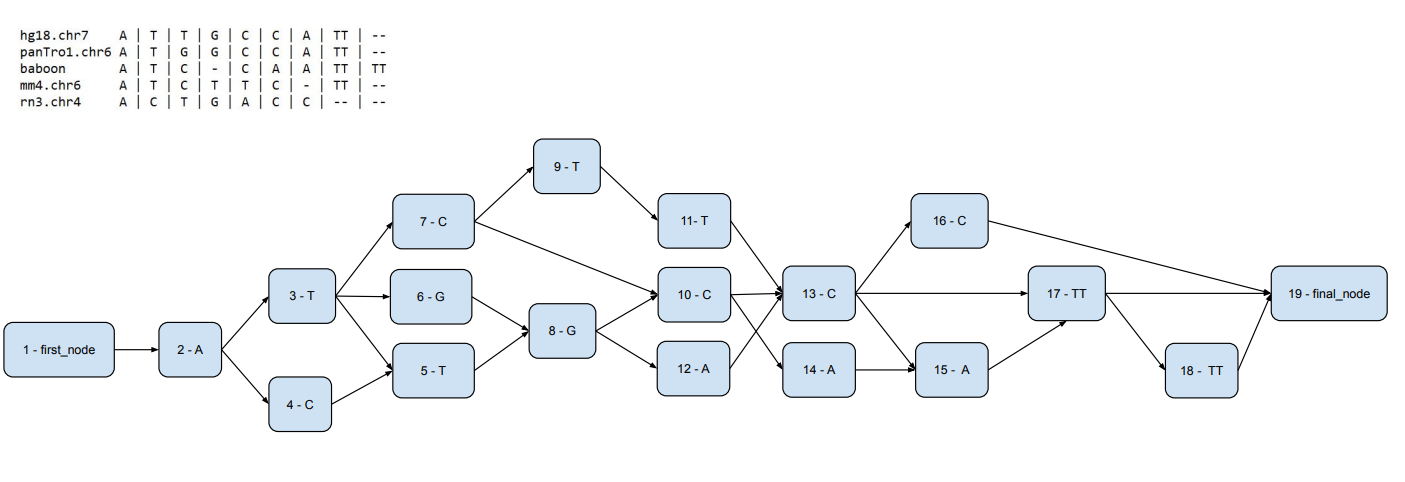
\includegraphics[scale=0.55]{images/Spling graph example.PNG}
    \caption{Esempio di Splicing graph, creato dal mio programma, con l'allineamento multiplo di riferimento}
    \label{fig:slicing_graph_example}
\end{figure}

Non tutti i percorsi $First\_node \to Last\_node$ corrispondo agli effettivi trascritti del gene. Sarebbe necessario limitare il numero di questi falsi trascritti.

\section{Costruzione dello Splicing Graph}
Mi è stato richiesto di implementare una libreria che permetta di creare un grafo di splicing.

In input è fornito un allineamento multiplo di trascritti per fare in modo di evidenziare le omologie tra le isoforme di splicing al fine di rendere più agevole la creazione del grafo. Sono state utilizzate due librerie esterne che permettono di costruire un \textit{Variation Graph} (una generalizzazione dello Splicing Graph) ed eseguire il parsing di file FASTA, uno dei formati standard in bioinformatica, per ottenere l'allineamento multiplo. 

Il parsing di file in formato MAF (Multiple Alignment Format), un altro formato standard in bioinformatica, in assenza di un'alternativa migliore, è stato da me implemementato a partire da una libreria incompleta che lo eseguiva parzialmente.

Nel prossimo capitolo saranno dati i dettagli della soluzione proposta.